\documentclass[xcolor=pdftex,dvipsnames,table]{beamer}
\usepackage[utf8]{inputenc}
\usepackage[misc]{ifsym}
\usepackage{textpos,tikz,calc,wasysym,xmpmulti}

% \usepackage{beamerthemesplit}
\usetheme{Copenhagen}
% \usecolortheme{structure}
\usefonttheme{professionalfonts}
\setbeamercolor{structure}{fg=black}


\title{Data gathering for the \emph{Humanitude} project}
\author{Krohg, Bård-Kristian}
\date{December 6th, 2017}


\begin{document}
\maketitle

\begin{frame}
  \frametitle{Introduction}
  
  \begin{columns}[c]
    \column{.75\textwidth}
    \begin{itemize}
    \item[] Bård-Kristian Krohg 
    \item[] University of Oslo / Kyushu University
    \item[] Academic advisors:\begin{itemize}
    \item[] Vice Dean, Professor, Kurazume Ryo 
    \item[] Professor, Jim Tørresen
    \end{itemize}
    \item[] \Letter \hspace{.3em} \texttt{baardkrk@student.matnat.uio.no} 
    \item[] Country of Origin: Norway
    \end{itemize}

    \column{.25\textwidth}
    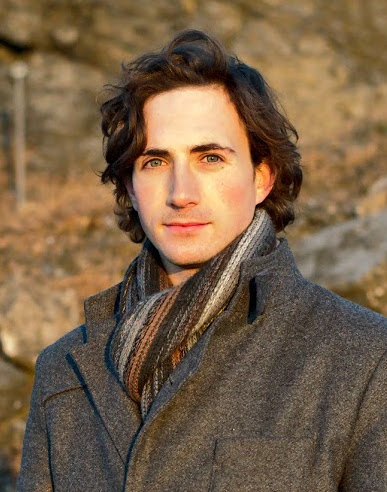
\includegraphics[width=\linewidth]{graphics/selfie.jpg}
  \end{columns}
\end{frame}

\begin{frame}
  \frametitle{Humanitude}
  
  The Japanese Ministry of Health, Labour and Welfare are evaluating the multimodal comprehensive care methodology called \emph{Humanitude}.\\
  \vspace{.7em} \pause
  Core elements: \\
  \begin{itemize}
  \item Eye contact
  \item Verbal communication
  \item Touch
  \end{itemize}\pause

  A preliminary case study~\cite{hindawi2016case} found patients more accepting of care when treated according to the \emph{Humanitude} method.\\

\end{frame}


\begin{frame}
  \frametitle{Teaching Assistant\\{\small Automated feedback system for trainees in \emph{Humanitude}}}
  Using data gathered from a skilled practitioner of \emph{Humanitude} we hope to provide useful feedback to a trainee.\\
  \vspace{1em} \pause
  \begin{columns}[t]
    \column{.48\textwidth}
    \textbf{Measuring selected features:}
    \begin{itemize}
    \item Posture
    \item Eye contact/motion
    \item Facial expression
    \item Tone of voice
    \item etc.
    \end{itemize} \pause
    \column{.48\textwidth}
    \textbf{Technologies:}
    \begin{itemize}
    \item Multiple RGB-D cameras
    \item OpenPose~\cite{cao2017realtime}
    \item People Localization and Tracking
    \end{itemize}
  \end{columns}
  
\end{frame}

\begin{frame}
  \frametitle{Sources}
  \bibliography{sources}
  \bibliographystyle{plain}
\end{frame}
\end{document}
